\chapter{Logic Implementation with JavaScript} \label{chapter:desgin}

The logic of this app is divided into two parts. First part is JavaScript logic, that is responsible for the functionalities of each HTML site, more precisely the dynamic response to the user. Second part is Java Android logic, which is responsible for the main function called tracking and all other functionalities that could not be accomplished with help of JS. 
\\

Altogether there are 10 html sites and each one of them has some functionalities that had to be implemented with JS or Android Java. A simple example of a functionality is clicking on a button that triggers a function that was declared inside the HTML site.
\\

However, JavaScript and Android Java doesn't provide everything that has been needed for the application. That's the reason why the project members had to use several other web frameworks like jQuery or phonegap.js to accomplish the main goal of powerful, user-friendly mobile application. The usage of web frameworks will be explained in further chapters. 

\section{Start Menu}
At the beginning of the application a start menu is displayed. In this menu the user can use functions that had been specially developed for this application. Functions like help, car tracking, favourite list, about and exit.
\\

\begin{figure}
\centering
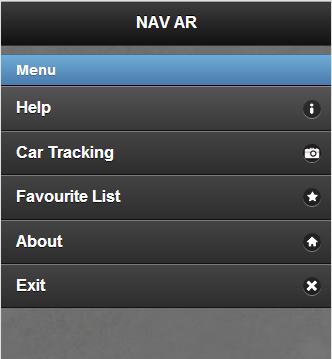
\includegraphics[width=0.6\linewidth]{graphics/chapter4/1}
\caption{Start menu of the application}
\label{fig:1}
\end{figure}
\newpage

Each one of these buttons have their logic that is implemented in index.html. The quell code x.x  shows the functionality behind each button.
\\

\begin{lstlisting}[language=html, caption= 
start menu source code,captionpos=b]
<li data-icon="info" ><a  href="help.html" rel="external">Help</a></li>
<li data-icon="camera"><a href="#" onclick="trackClick();">Car Tracking</a></li>
<li data-icon="star" ><a href="myfavourite.html" rel="external">Favourite List</a></li>
<li data-icon="home" ><a href="about.html" rel="external">About</a></li>
<li data-icon="delete"><a href="#" onclick="turnOff();">Exit</a></li>
\end{lstlisting}

\
Functions trackClick() and turnOff() were implemented in Android Java and are described in chapter 
\
\
\begin{lstlisting}[language=html, caption= 
JS start menu methods,captionpos=b]
function trackClick() {
    MyTracking.performClick();
}

function turnOff(){
	Exit.exitClick();
}
\end{lstlisting}

The button "help" forwards the user  to the help display (help.html). The same functionality features about and favourite list, except they link on to different displays. 
\\

"Exit" button invokes the function turnOff() calls another Android Java implemented function. "Exit.exitClick()" ends the app. Look at fig. x.x.x
\\

"Car tracking" calls a function named "trackClick()". As "Exit" it requests another Android Java impl method. This method starts the tracking.
\\

\section{Help}

The help display provides only two major options: back button and the link to the self created YouTube video. 


\begin{figure}[b]
\centering
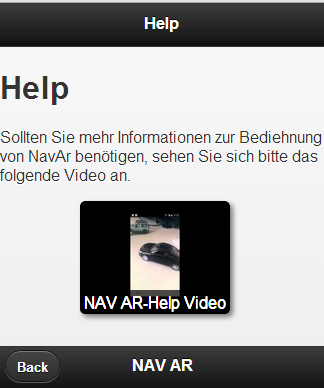
\includegraphics[width=0.5\linewidth]{graphics/chapter4/2}
\caption{}
\label{fig:2}
\end{figure}
\newpage

The back button leads back to the main menu. Illustrated in figure x.x
\\
\begin{lstlisting}[language=html, caption= 
back button,captionpos=b]
<a class="ui-btn-left" href="index.html" rel="external">Back</a>
\end{lstlisting}
\
\
If the user presses the picture "HAV AR-Help Video" he will be linked to a specific YouTube video that has been created by the project team. This video serves as a how to. It shows how to use the applications main functions.
\\
\begin{lstlisting}[language=html, caption= 
help video,captionpos=b]
<ul id="Gallery" class="youtube-videogallery" align="center">
<li><a href="https://www.youtube.com/watch?v=6U4oT5AbAsg&feature=youtu.be">NAV AR-Help Video</a></li>
</ul>
\end{lstlisting}

\section{Start Menu}
The most important function of the hole mobile applications is tracking. This function is executed by "MyTracking.peformClick()". More in chapter 4.1)Start Menu.
\\

After the car was successfully tracked, the user is linked to a new display called "index.html". This display or better called start menu, provides the user with additional options. Options that deliver information as well review about the tracked car and other useful functions. 
\\

There is also a possibly to add the tracked car to users collection named the favourite list. Out of the favourite list the user can select one specific vehicle to use start menu options, like pictures or videos about that specific car.  
\\

JavaScript functions had to be created for each start menu options. These functions are described in chapter 4.3.1)JavaScript Functions.
\\

\begin{figure}[]
\centering
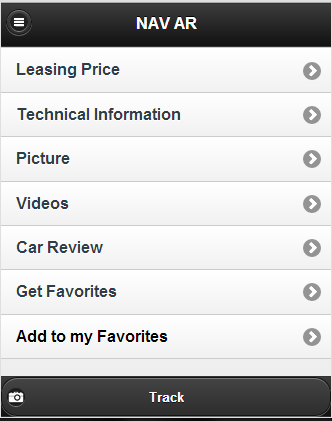
\includegraphics[width=0.5\linewidth]{graphics/chapter4/3}
\caption{}
\label{fig:3}
\end{figure}
\newpage

\subsection{JavaScript Functions}



\subsubsection{Start Timer}
When the site is loaded a timer automatically starts. Specific functions stop the timer and sends the time to the Navision server.
\\
\begin{lstlisting}[language=html, caption= 
start timer function,captionpos=b]
function startTime(){
	var d = new Date();
	timestart = d.getTime();
}
\end{lstlisting}

\subsubsection{End Timer}
This function stop the timer which had been started with the method startTime() and safes the time with the method timestampsave() into the server. Start time and end time were used to get the time how long a user has selected a specific car.
\\
\begin{lstlisting}[language=html, caption= 
start timer function,captionpos=b]
function endtime(){
        var d = new Date();
        var endtime = d.getTime();
        timestampsave(timestart,endtime);
    }
\end{lstlisting}


\subsubsection{Save time stamp}
This function saves start time and end time of the timer, into the Navision server. The start time and end time are input parameters. 
\\

To save the time into the server timestampsave() needs several other information like email and id of the tracked car. More about sending information to the server and the connectivity between application and server go to the chapter
\\

time1..start time

time2..end time
\\
\begin{lstlisting}[language=html, caption= 
start timer function,captionpos=b]
function timestampsave(time1,time2){
        var stime	= 	time1;
        var endtime	=	time2;
        var emailan = 	sessionStorage.getItem('email');
        var fid 	= 	sessionStorage.getItem('id');
        

        $(document).ready(function () {
            $.ajax({
                type: "GET",
                url: "http://ar-tgm-navax.cloudapp.net:9090/rest/insertTrackingHistory/"+emailan+"/"+fid+"/"+stime+"/"+endtime+"/ac73f229f1fb88a8719e5f6d295bee45?callback=?",
                async: false,
                dataType: 'JSONP',
                success: function(data){
                    //do your stuff with the JSON data
                    var test=data;
                    console.log(test);
                }
            });
        });
    }
\end{lstlisting}


\subsubsection{Set Parameters}
There are two parameters that have to be saved into the session storage to use several other functions and the connection from client app to Navision server.
\\
\begin{lstlisting}[language=html, caption= 
start timer function,captionpos=b]
function setParam(){
	window.sessionStorage.setItem('id', myVariable);
	window.sessionStorage.setItem('email',email);
}
\end{lstlisting}




\subsubsection{Start Tracking}
This function starts to track a car. For more explanation refer to chapter "Implementation in Android Java and Metaio Tracking"
\\

\begin{lstlisting}[language=html, caption= 
start timer function,captionpos=b]
function trackClick() {
        MyTracking.performClick();
    }
\end{lstlisting}

\subsubsection{Review}
This method is implemented with Java Android. More about in chapter "Implementation in Android Java and Metaio Tracking"
\\
\begin{lstlisting}[language=html, caption= 
start timer function,captionpos=b]
function reviewClick(){
        Review.performClick();
    }
\end{lstlisting}


\subsubsection{Turn off}
This function is implemented with Java Adroid and has been documented in 4.1)Start Menu.
\\

\begin{lstlisting}[language=html, caption= 
start timer function,captionpos=b]
function turnOff(){
        Exit.performClick();
    }
\end{lstlisting}



\subsubsection{Home}
This function returns the user back to the start menu. This function is coupled with the button Home. Also implemented with Java Android.
\\

\begin{lstlisting}[language=html, caption= 
start timer function,captionpos=b]
function home(){
        Home.performClick();
    }
\end{lstlisting}


\subsubsection{Read car name}
This method returns the name of the car that had been tracked threw a car specific id. Each transport has its own unique id. This id is set after the tracking and is stored in session storage.  So the input parameter "cname" is that specific id of the tracked or out of favourite list selected car. The name of the car is stored on the Navision server. A request had to be send to receive the name. More about Connectivity in chapter coming soon 
\\

\begin{lstlisting}[language=html, caption= 
start timer function,captionpos=b]
function readcarname(cname){
        var test = '';
        $(document).ready(function () {
            $.ajax({
                type: "GET",
                url: "http://ar-tgm-navax.cloudapp.net:9090/rest/getKFZInfo/"+cname+"/ac73f229f1fb88a8719e5f6d295bee45?callback=?",
                async: false,
                dataType: 'JSONP',
                success: function(data){
                    test=data.split(';');
                    globalcarname=test[0];
					document.getElementById("add_favorite").style.color="black";
                }
            });

        });
    }
\end{lstlisting}


\subsubsection{Save email}
As the name says, saveEmail() saves the email of the user. The information about users email was already stored in session storage through the function "setParam()". Now this email is read out of the session storage and is going to be stored into the Navision server. More about connection between app and server read coming soon.
\\

\begin{lstlisting}[language=html, caption= 
start timer function,captionpos=b]
function saveEmail(){    
        var value3 = sessionStorage.getItem('email');
        
        $(document).ready(function () {
            $.ajax({
                type: "GET",
                url: "http://ar-tgm-navax.cloudapp.net:9090/rest/insertAndroidEmail/"+value3+"/ac73f229f1fb88a8719e5f6d295bee45?callback=?",
                async: false,
                dataType: 'JSONP',
                success: function(data){
                    //do your stuff with the JSON data
                    var test=data;
                    console.log(test);
                }
            });
        });

\end{lstlisting}

\subsubsection{Save car}
This function saves the id and the name of the tracked auto. This method is used for adding new cars to users favorites.  In this function a feature that provides HTML5 for its users was used. The function can be split into 4 phases.
\\

Phase one checks if the input parameter "name" is not empty. If it is empty usere receives information about it, otherwise it proceives with other phases

\begin{lstlisting}[language=html, caption= 
start timer function,captionpos=b]
if(name!=null){
.....
}else{
alert("Function is loading due to slow internet connection.");
}
\end{lstlisting}

Phase two is the search for unique local storage place with specific name(favorites, fcarna) and inspecting if this storage exists or not. If it doesn't exists an empty string is put inside the two local storages, otherwise nothing is done.
\\

\begin{lstlisting}[language=html, caption= 
start timer function,captionpos=b]
ifif ((localStorage.getItem("favorites") === null) && (localStorage.getItem("fcarname") == null)) {
	var names = [];
	localStorage["favorites"] = JSON.stringify(names);
	localStorage["fcarname"] = JSON.stringify(names);
}
\end{lstlisting}

In phase three variables storedIds and storedNames are filled with information inside the local storage "favorites" and "fcarname".
\\

\begin{lstlisting}[language=html, caption= 
start timer function,captionpos=b]
var storedIds = JSON.parse(localStorage["favorites"]);
var storedNames = JSON.parse(localStorage["fcarname"]);
\end{lstlisting}

Phase four checks if the new car not already exists inside the local storage. If the car exists user receives information that this car already exists in his favourite list, otherwise the id and car name is saved into the local storage.
\\

\begin{lstlisting}[language=html, caption= 
start timer function,captionpos=b]
if (storedIds.indexOf(id) > -1) {
	Notifier.error('Car already exists.');
}else{
	storedIds.push(id);
	storedNames.push(name);
	localStorage["favorites"] = JSON.stringify(storedIds);
	localStorage["fcarname"] = JSON.stringify(storedNames);
	Notifier.success('Car has been added.');
}
\end{lstlisting}

The abb x.yy shows the hole function with its four phases.
\begin{lstlisting}[language=html, caption= 
start timer function,captionpos=b]
function LocalStorageWriteId(id,name){
		if(name!=null){
			if ((localStorage.getItem("favorites") === null) && (localStorage.getItem("fcarname") == null)) {
				var names = [];
				localStorage["favorites"] = JSON.stringify(names);
				localStorage["fcarname"] = JSON.stringify(names);
			}
			
			var storedIds = JSON.parse(localStorage["favorites"]);
			var storedNames = JSON.parse(localStorage["fcarname"]);
		
			if (storedIds.indexOf(id) > -1) {
				Notifier.error('Car already exists.');
			}else{
				storedIds.push(id);
				storedNames.push(name);
				localStorage["favorites"] = JSON.stringify(storedIds);
				localStorage["fcarname"] = JSON.stringify(storedNames);
				Notifier.success('Car has been added.');
			}
		}else{
			alert("Function is loading due to slow internet connection.");
		}
    }
\end{lstlisting}

\subsection{Used Functionalities}
In functions that were created extra for mainmenue.html were several new features and functionalities used. In this chapter all functionalities will be described 
\\

\subsubsection{Session Storage}
Moreover ,the function called Sessionstorage has a big importance in this project. The Sessionstorage saves the value not persist, that means if the App is closed or has been ended so the value will be wiped of . In the next Session or if the App has been started , there will be then a new Sessionstorage. In this case the Project NAVAR uses the Sessionstorage to save the ID from the car which has been tracked. Sessionstorage allows  to save a large amount of  key/value pairs and lots of text. This feature is impossible to do it via cookie. This kind of functionality uses  a protocol to save the Data. This protocol checks if the key and value is a string, but if not it convert them to a string. Furthermore if a key was already present, its entry  has to be removed and the new one will be appended. The sessionStorage has it own methods for specific functionality.
First one is method is used to tell how many key/pair the SessionStorage contains. This method is same function ,which tells the length of an Array.

\subsubsection{Local Storage}

HTML 5 provides us with a new feature called Web Storage. In other words, with HTML5, web pages can store data locally within the user's browser.
\\

Earlier, this was done with cookies. However, Web Storage is more secure and faster. The data is not included with every server request, but used ONLY when asked for. It is also possible to store large amounts of data, without affecting the website's performance.
\\

The data is stored in name/value pairs, and a web page can only access data stored by itself. Unlike cookies, the storage limit is far larger (at least 5MB) and information is never transferred to the server.
\\

HTML5 Web Storage provides two new objects for storing data on the client:
\begin{enumerate}
\item window.localStorage - stores data with no expiration date
\item code.sessionStorage - stores data for one session (data is lost when the tab is closed)
\end{enumerate}
\newpage

\begin{figure}[t]
\centering
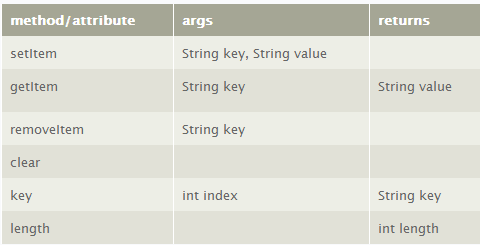
\includegraphics[width=0.9\linewidth]{graphics/chapter4/20}
\caption{}
\label{fig:4}
\end{figure}


Here is an example of setItem and getItem in local storage.
\\

\begin{lstlisting}[language=html, caption= 
start timer function,captionpos=b]
var foo = localStorage.getItem("bar");
// ...
localStorage.setItem("bar", foo);
\end{lstlisting}

In these application not a string but an array is stored inside the local storage. Here is an example how we put an empty array into a local storage.
\\

\begin{lstlisting}[language=html, caption= 
start timer function,captionpos=b]
var names = [];
localStorage["favorites"] = JSON.stringify(names);
\end{lstlisting}

And so was the array received from the local storage called favourites".
\\
\begin{lstlisting}[language=html, caption= 
start timer function,captionpos=b]
var storedIds = JSON.parse(localStorage["favorites"]);
\end{lstlisting}

\subsubsection{AJAX}
More about AJAX in chapter AJAX
\\

\subsection{GUI}
The GUI provides the user with 8 operations and one slide panel. Each operation is a butten which invokes self created functions that are described in chapter 4.3.1)Created Functions.
\\
\begin{lstlisting}[language=html, caption= 
start timer function,captionpos=b]
<ul data-role="listview" >	
            <li><a href="leasingprice.html" rel="external">Leasing Price</a></li>
            <li><a href="technicalinfo.html" rel="external">Technical Information</a></li>
            <li><a href="slide.html"  data-transition="slide" rel="external">Picture</a></li>
            <li><a href="video.html" rel="external">Videos</a></li>
            <li><a href="#" rel="#"  onclick="reviewClick();">Car Review</a></li>
            <li><a href="myfavourite.html"rel="external" >Get Favorites</a></li>
			<li><a id="add_favorite" onclick="LocalStorageWriteId(sessionStorage.getItem('id'),globalcarname);" style="color:red" rel="external" >Add to my Favorites</a></li>
</ul>
\end{lstlisting}


\begin{figure}[H]
\centering
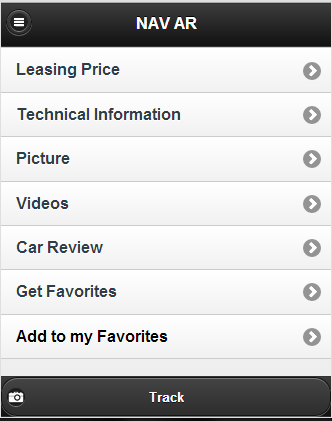
\includegraphics[width=0.4\linewidth]{graphics/chapter4/4}
\caption{}
\label{fig:5}
\end{figure}
\newpage

\subsubsection{Leasing Price}
\
When the user clicks on the butten Leasing price he is going to be linked to the html page "leasingprice.html" where he receives informations about the price of the tracked vehicle.

\begin{figure}[H]
\centering
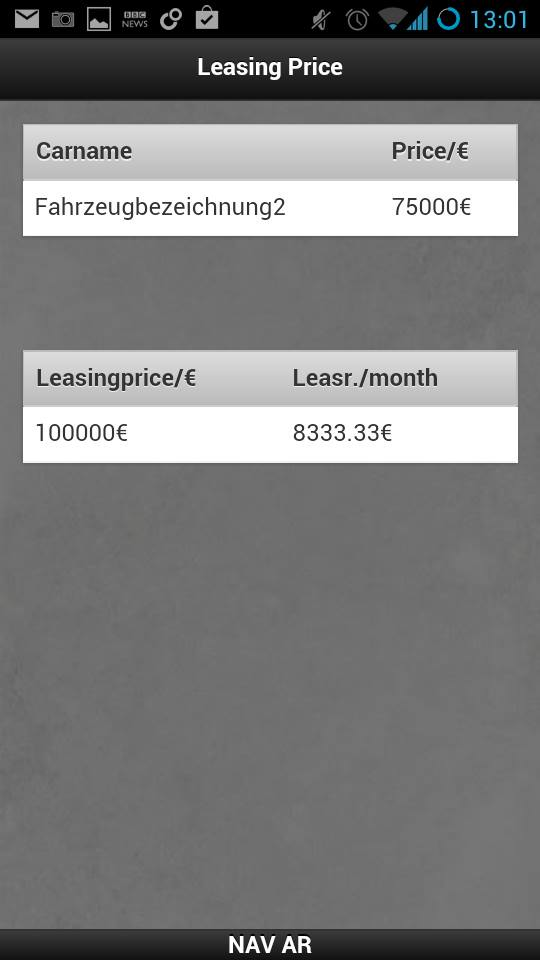
\includegraphics[width=0.4\linewidth]{graphics/chapter4/5}
\caption{}
\label{fig:6}
\end{figure}


\subsubsection{Technical Information}
As leasing price it also only links to another html site called "technicalinfo.html". In this page several features were used. Phone Gallary and Dynamic Selection of Colour. Informations about those features are in chapters LOl
\\
\begin{figure}[H]
\centering
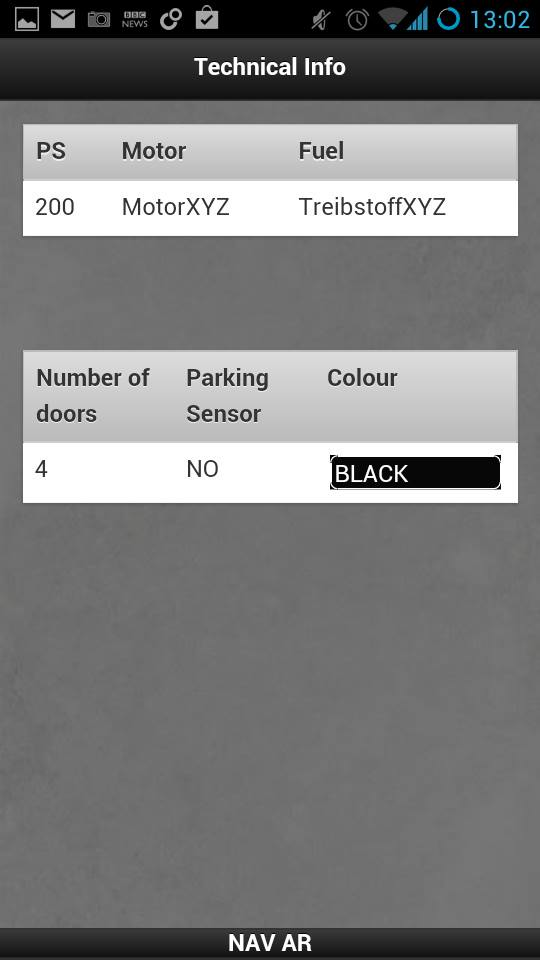
\includegraphics[width=0.4\linewidth]{graphics/chapter4/6}
\caption{}
\label{fig:7}
\end{figure}
\newpage

\subsubsection{Pictures}
Operations pictures links to a site "slide.html" that shows several modern pictures of tracked car. Feature called Photo Gallary in chapter "Design Concept" was used inside that site.
\\
\begin{figure}[H]
\centering
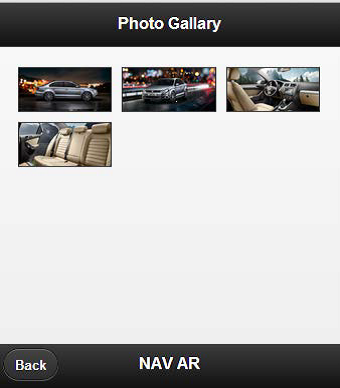
\includegraphics[width=0.5\linewidth]{graphics/chapter4/7}
\caption{}
\label{fig:8}
\end{figure}
\newpage

\subsubsection{Videos}
Operation videos links to a page called video.html. This page provides user with videos about the selected car from favourite list or fresh tracked one. More about video gallery in chapter "Design Concep"
\\
\begin{figure}[H]
\centering
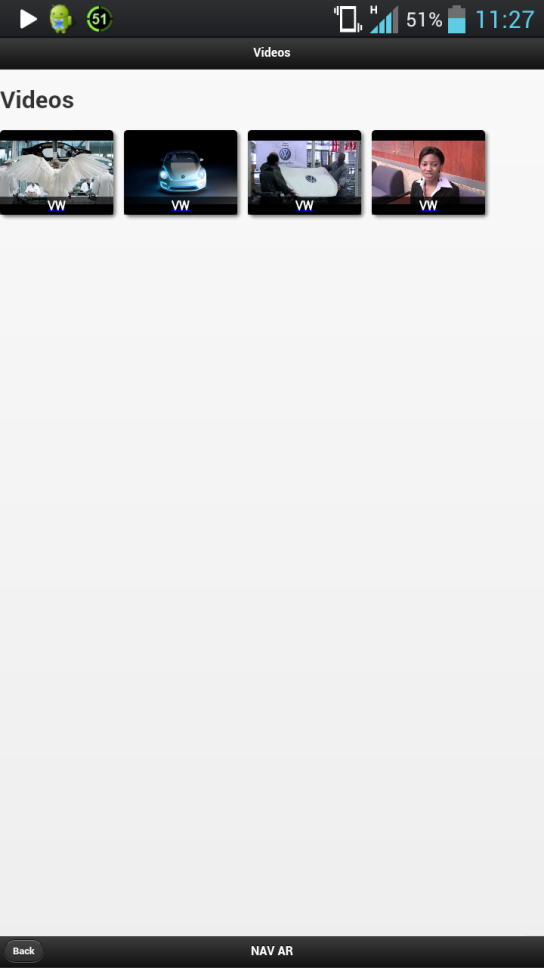
\includegraphics[width=0.5\linewidth]{graphics/chapter4/8}
\caption{}
\label{fig:9}
\end{figure}
\newpage

\subsubsection{Review}
Operation review invokes a self created method called reviewClick(). Description to this method is in chapter 4.3.1 Created Methods, Review. Basicly review links the user to a new site where he can read review about the specific car.
\\
\begin{figure}[H]
\centering
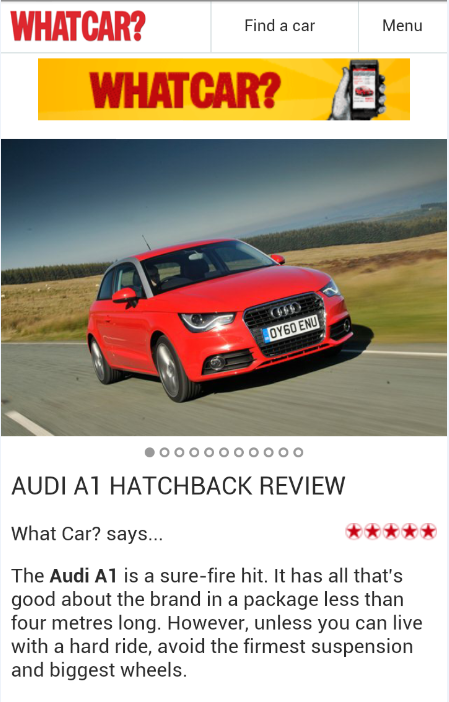
\includegraphics[width=0.5\linewidth]{graphics/chapter4/9}
\caption{}
\label{fig:10}
\end{figure}
\newpage


\subsubsection{Get Favourites}
This operations links the user to his favourite cars which he saved with the operation "add to my favourite". Information about the favourite list in chapter 4.4)My Favourites.
\\
\begin{figure}[H]
\centering
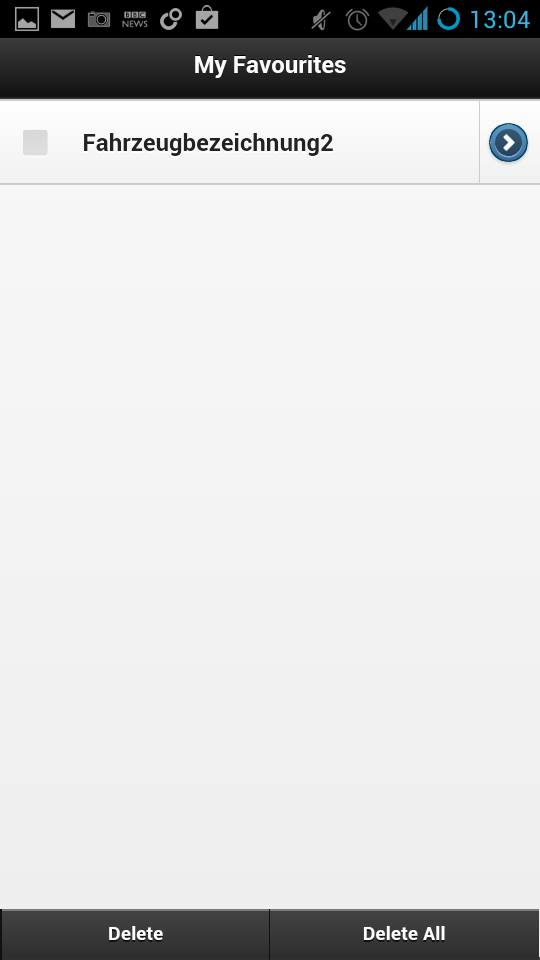
\includegraphics[width=0.5\linewidth]{graphics/chapter4/10}
\caption{}
\label{fig:11}
\end{figure}
\newpage

\subsubsection{Add to my Favourites}
The button "Add to my Favourites" trigger the function LocalStorageWriteId. This function saves the id and the name of the tracked car into users favourites. For the first param it takes the tracked car id from the session storage. As the second parameter the global variable globalcarname.
\\
\begin{lstlisting}[language=html, caption= 
start timer function,captionpos=b]
<li><a id="add_favorite" onclick="LocalStorageWriteId(sessionStorage.getItem('id'),globalcarname);" style="color:red" rel="external" >Add to my Favorites</a></li>
\end{lstlisting}
Before the user can add the vehicle to his favourite he has to wait several seconds. In this time the request is send to the server to get information about the car threw its id. If the user wants to access the operation in its loading time, the application denies him the acces and informs him about the loading time.
\\
\begin{figure}[H]
\centering

\includegraphics[width=0.6\linewidth]{graphics/chapter4/11}
\caption{}
\label{fig:12}
\end{figure}

The operations colour changes from red to block when the operations is loaded.
\\
\begin{figure}[H]
\centering

\includegraphics[width=0.6\linewidth]{graphics/chapter4/12}
\caption{}
\label{fig:13}
\end{figure}


\subsection{Slide Panel}
In the upper left corner of the display exists a small button which calls the slide panel to open. More about slide panel itself read in chapter.
\\
\begin{figure}[H]
\centering
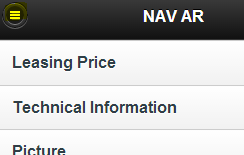
\includegraphics[width=0.4\linewidth]{graphics/chapter4/13}
\caption{}
\label{fig:14}
\end{figure}

If the user calls this button a slide panel with more functions will be shown.
\\
\begin{figure}[H]
\centering
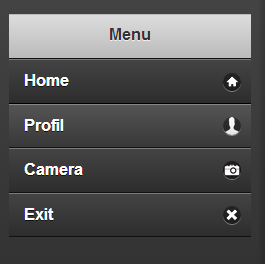
\includegraphics[width=0.4\linewidth]{graphics/chapter4/14}
\caption{}
\label{fig:15}
\end{figure}
\newpage
Here has the user four new options. He can return to the start menu with the display home, or he can accesses his profile. Also he can start to track a new car with camera. If the user doesn't want use the mobile application anymore, he can close it the button exit. 
\\
\begin{lstlisting}[language=html, caption= 
start timer function,captionpos=b]
<ul data-role="listview" data-theme="a" >
                <li data-icon="home" ><a href="#" onclick="endtime();home();">Home</a></li>
                <li data-icon="profil"><a href="profile.html" rel="external" >Profil</a></li>
                <li data-icon="camera" ><a href="#" onclick="endtime();trackClick();">Camera</a></li>
                <li data-icon="delete"><a href="#" onclick="endtime();turnOff();">Exit</a></li>
</ul>
\end{lstlisting}

The home button not only returns the user to the start menu but also ends the timer that has been started after a car was tracked. In addition, this time is send straight to the Navision server.  
\\

Display profil calls to another display called profile.html, where the user can see his profile data. 
Camera function ends the timer and starts the tracking function. Exit ends the application.



\section{My Favourites}
\begin{figure}[H]
\centering
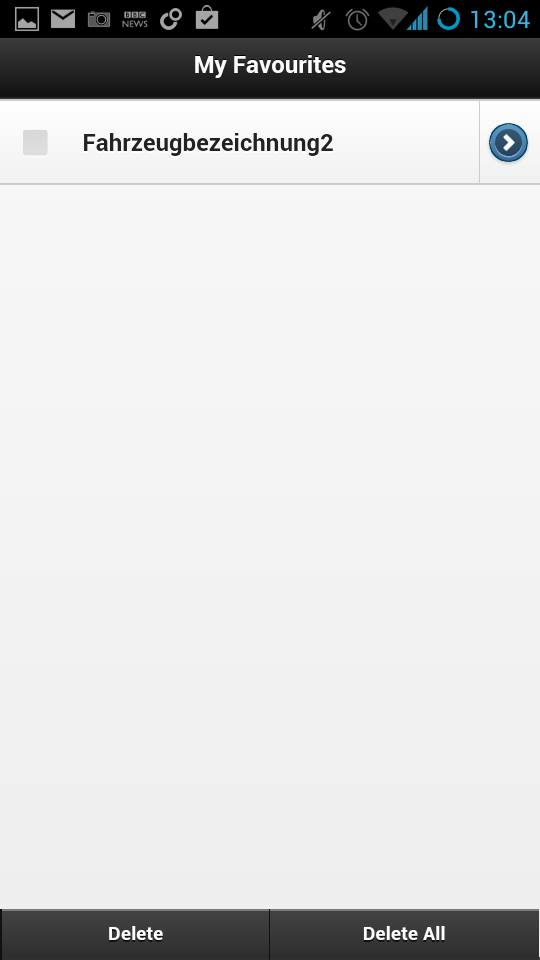
\includegraphics[width=0.4\linewidth]{graphics/chapter4/15}
\caption{}
\label{fig:16}
\end{figure}

Inside the favourites are cars had been added threw the operation add to my favourites. The favourite cars can be selected or deleted. Removing the cars from favourites is possible by selecting the specific vehicle or removing all of the cars.
\\

\subsection{Loading of favourite cars}
Before the functions of the favourite list can be used, the list entries(cars) have to be initialized. This is done automatically when the site is loaded. Each line that is written inside document.ready starts after the document is ready. This is where the favourite cars are initialized.
\\
\begin{lstlisting}[language=html, caption= 
start timer function,captionpos=b]
$(document).ready(function () {
.
.
});
\end{lstlisting}

First, all car names are loaded from local storage into an array called storedCarNames. So this array is filled with vehicle names which user added to his favourites. 
\\

\begin{lstlisting}[language=html, caption= 
start timer function,captionpos=b]
var storedCarNames = JSON.parse(localStorage["fcarname"]); 
\end{lstlisting}

Now the filling of the cars into a list begins. The loop goes so long as the number of cars are in the array. In this loop a car name is put into the litItem1 which is just a panel shown in ref x.x
\\

Next listItem1 is put into another list. This list is where all panels(favourite cars) are stored. Each new vehicle is put into the list. It is dope with the line.
\\
\begin{lstlisting}[language=html, caption= 
start timer function,captionpos=b]
for (var i = 0; i < storedCarNames.length; i++)  
         {
             var key = storedCarNames[i];

            listItem1 = '<li><a style="padding-top: 0px;padding-bottom: 0px;padding-right: 42px;padding-left: 0px;">' +
                    '<label style="border-top-width: 0px;margin-top: 0px;border-bottom-width: 0px;margin-bottom: 0px;border-left-width: 0px;border-right-width: 0px;" data-corners="false">' +
                    '<fieldset data-role="controlgroup" >' +
                '<input id="' + i + '" name="SelectedSensors[0].Value" type="checkbox" value="true" />' +
                '<input id="SelectedSensors_0__Id" name="SelectedSensors[0].Id" type="hidden" value="16" />' +
                '<label for="SelectedSensors_0__Value" style="border-top-width: 0px;margin-top: 0px;border-bottom-width: 0px;margin-bottom: 0px;border-left-width: 0px;border-right-width: 0px;">' +
                '<label  style="padding:10px 0px 0px 10px;">' +
                key +
                '</label>' +
                '</label>' +
                ' </fieldset>' +
            '</label>' +
            '</a><a onclick="EventHandler();" href="mainmenue.html" rel="external"></a>' +
            '</li>';

            $('#liste').append(listItem1);
         }
\end{lstlisting}

\begin{figure}[H]
\centering

\includegraphics[width=0.4\linewidth]{graphics/chapter4/16}
\caption{}
\label{fig:17}
\end{figure}

Last but not least the liste has to be refreshed so the listItems are used. 
\\

\begin{lstlisting}[language=html, caption= 
start timer function,captionpos=b]
$('#liste').listview('refresh').trigger('create'); 
\end{lstlisting}

\subsection{JS Functions}
\subsubsection{Delete favourite car}
This method deletes selected car with help of check box. If no car is selected, nothing happens.
\\
\begin{lstlisting}[language=html, caption= 
start timer function,captionpos=b]
function deleteF(){
	
	Array.prototype.clean = function(deleteValue) {
  		for (var i = 0; i < this.length; i++) {
    		if (this[i] == deleteValue) {         
      			this.splice(i, 1);
				i--;
			}
		}
		return this;
	};
	
	var storedNames = JSON.parse(localStorage["favorites"]); //the ids of cars
    var storedCarNames = JSON.parse(localStorage["fcarname"]); //the names of cars
	var lengthof=0;

	for(var s=0;s<storedNames.length;s++){
		if(document.getElementById(s).checked){
			delete storedNames[s];
            delete storedCarNames[s];
			lengthof++;
		}
		
	}
	if(lengthof!=0){
		Notifier.success('Cars deleted.');
	
		storedNames.clean(undefined);
		storedCarNames.clean(undefined);

		localStorage["favorites"] = JSON.stringify(storedNames);
		localStorage["fcarname"] = JSON.stringify(storedCarNames);
	}
	window.location.reload();
}
\end{lstlisting}

\subsubsection{Delete all favourite cars}
Removes all favourite cars without selecting them.

\begin{lstlisting}[language=html, caption= 
start timer function,captionpos=b]
function deleteAll(){
    Notifier.success('All cars have been deleted.');
	localStorage.clear();
    window.location.reload();
}
\end{lstlisting}

\subsubsection{Select favourite car}
Each car inside the favourite list can be selected. After the car is selected user is linked to the start menu.
\\

\begin{lstlisting}[language=html, caption=
start timer function,captionpos=b] 

function EventHandler() {
	Notifier.success('Car is selected.');
	var id = this.id;
	
	var storedNames = JSON.parse(localStorage["favorites"]);
	
	for(var i=0; i<storedNames.length;i++){
		if(id==i){
			window.sessionStorage.setItem('id', storedNames[i]);
		}
	}
}
\end{lstlisting}

\section{About}
The "about" page has no logic or no self made functions except one the back butten which functionality you have learnt in 4.2)Help chapter.
\\
\begin{figure}[H]
\centering
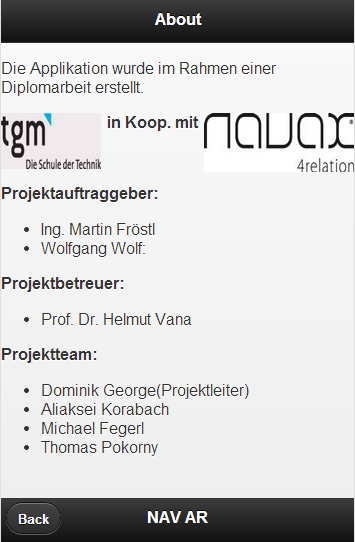
\includegraphics[width=0.4\linewidth]{graphics/chapter4/17}
\caption{}
\label{fig:18}
\end{figure}